\documentclass[12pt]{article}
\usepackage{setspace}
\doublespacing
\usepackage{fullpage}
\usepackage{amsbsy}
\usepackage{amsmath}
\usepackage{amsfonts}
\usepackage{amsthm}
\usepackage{amssymb}
\usepackage{algorithmic}
\usepackage{algorithm}
\usepackage{enumerate}
\usepackage{epsfig}
\usepackage{graphicx}
\usepackage{multirow}
%\usepackage{natbib}
\usepackage{xr}
\usepackage{color}
\usepackage{subfigure}
\numberwithin{equation}{section}

%%%%%%%%%%%%%%%%%%%%%%%%%%%%%%%%%%%%%%%%%%%%%%%%%%%%%%%%%%

\begin{document}

\title{\bf{Matrix Multiplication \\ CS 5220: Homework 1}}

\author{Group 9 \\ Ze Jin (zj58)\quad Sam Tung (sat83) \quad Patrick Cao (pxc2) \\}

\date{ }
%\date{\today}

\maketitle





\section{Method}

We refer to the tuning ideas on the note ``Tuning on a single core''.

\subsection{Blocking}

We can partition matrices into small blocks, and apply the block matrix multiplication.
\\
The advantage is that original matrices cannot fit into cache while the little blocks can.
\\
We compare different block sizes, including $2^p$, $1 \leq p \leq 10$.

\subsection{Loop Order}

In the naive implementation, we loop over $i$, then $j$, then $k$.
\\
An alternative loop order might be more cache friendly. For example, using the $(i, j, k)$ order, we have to go across a row of $A$ in the inner loop, which is a non-unit-stride access.

\subsubsection{Pure Loop Order}

From the original implementation, we access the following:
\begin{verbatim}
A[k*M + i]
B[j*M + k]
C[j*M + i]
\end{verbatim}
From a purely theoretical standpoint, the original loop order of $i,j,k$ may not be the most efficient, as matrix A is being iterated through by indices dependent on $k$ and $i$. This would imply that the loop should be reordered to have $k$ and $i$ be the innermost two loops, and $j$ be the outermost one.
\\
It should be noted that while this works in the initial implementation of matrix multiplication, if matrices are transposed, the loop ordering will need to be altered.

\subsubsection{Loop Order with Blocking}
We compare different orders, including $(i, k, j), (j, i, k), (j, k, i)$.
\\
When we apply blocking, there are two layers of loop orders. For example, the algorithm for looping order $(i, j, k)\times(j, i, k)$ is as follows.
\begin{verbatim}
for block i
    for block j
        for block k
            for cell j
                for cell i
                    for cell k
                        do calculation
\end{verbatim}
Again, we compare different combinations of block size and two-layer looping order.

\subsection{Copy Optimization}

We might run into conflict misses associated with cache. One way to solve the problem is to explicitly copy blocks into a contiguous block of local storage before multiplying them.
\\
Another side benefit of copy optimization is that we can use it to gracefully deal with fringe blocks.
\\
We add copy optimization to enhance blocking, and compare different block sizes, including $2^p$, $1 \leq p \leq 10$.

\subsection{Compiler Flag}

It is worthwhile playing with the flags that control the compiler optimizations, since modern compilers do some types of optimizations much better than people do.
\\
We compile the code with option \texttt{-funroll-loops} to unroll loops (basic loop unrolling is automatic with -O3).

\section{Result}

We run jobs on the totient cluster, and get the results depicted in several plots.

\subsection{Blocking}

See Figure 1 and 2 below for blocking with default loop order $(i, j, k)\times(i, j, k)$.
\\
The plot shows that blocking performs the best with block size $64, 128, 256$.

\begin{figure}[!ht]
   \begin{subfigure}
      \centering
        \begin{center}
      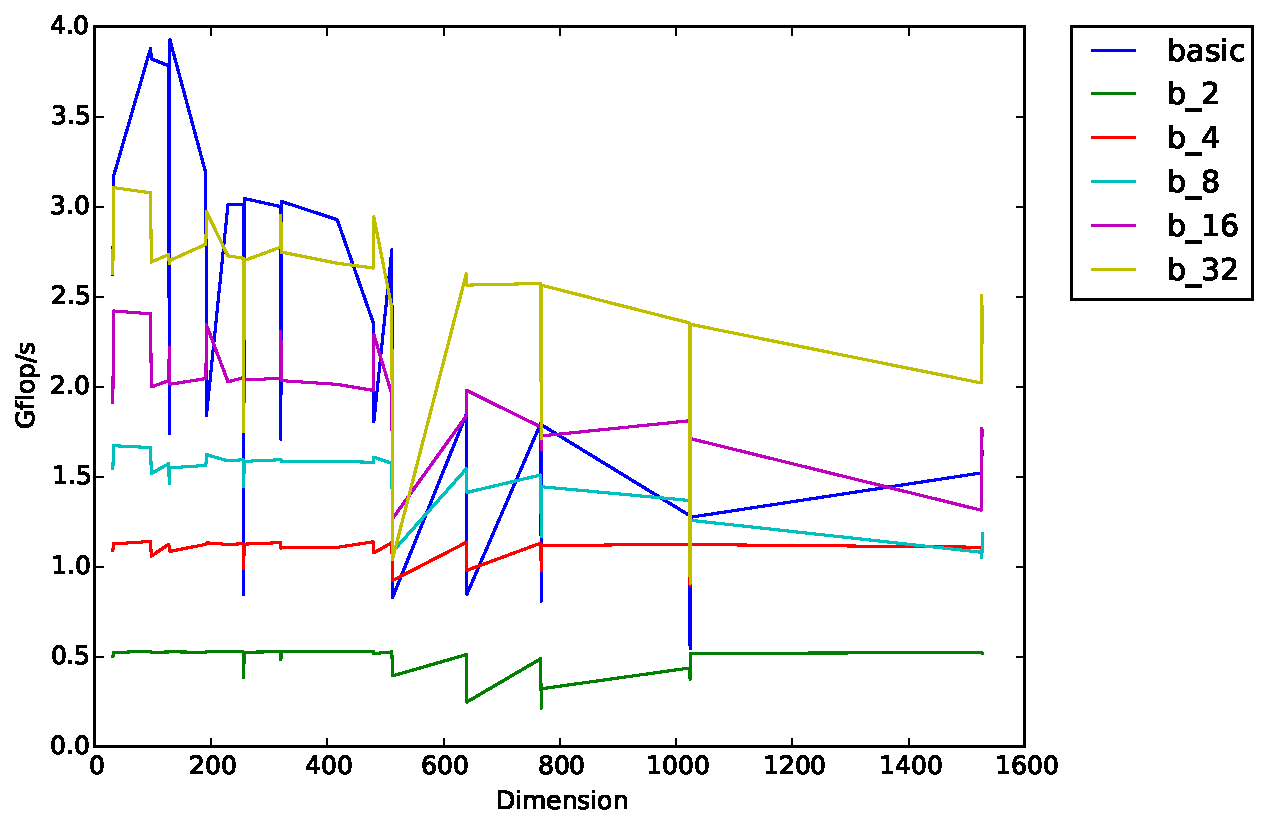
\includegraphics[width=0.85\textwidth] {timing_b_ijk_ijk_1}
        \end{center}
      \label{aload0}
      \caption{blocking with loop order $(i, j, k)\times(i, j, k)$}
  \end{subfigure}
  \begin{subfigure}
      \centering
        \begin{center}
      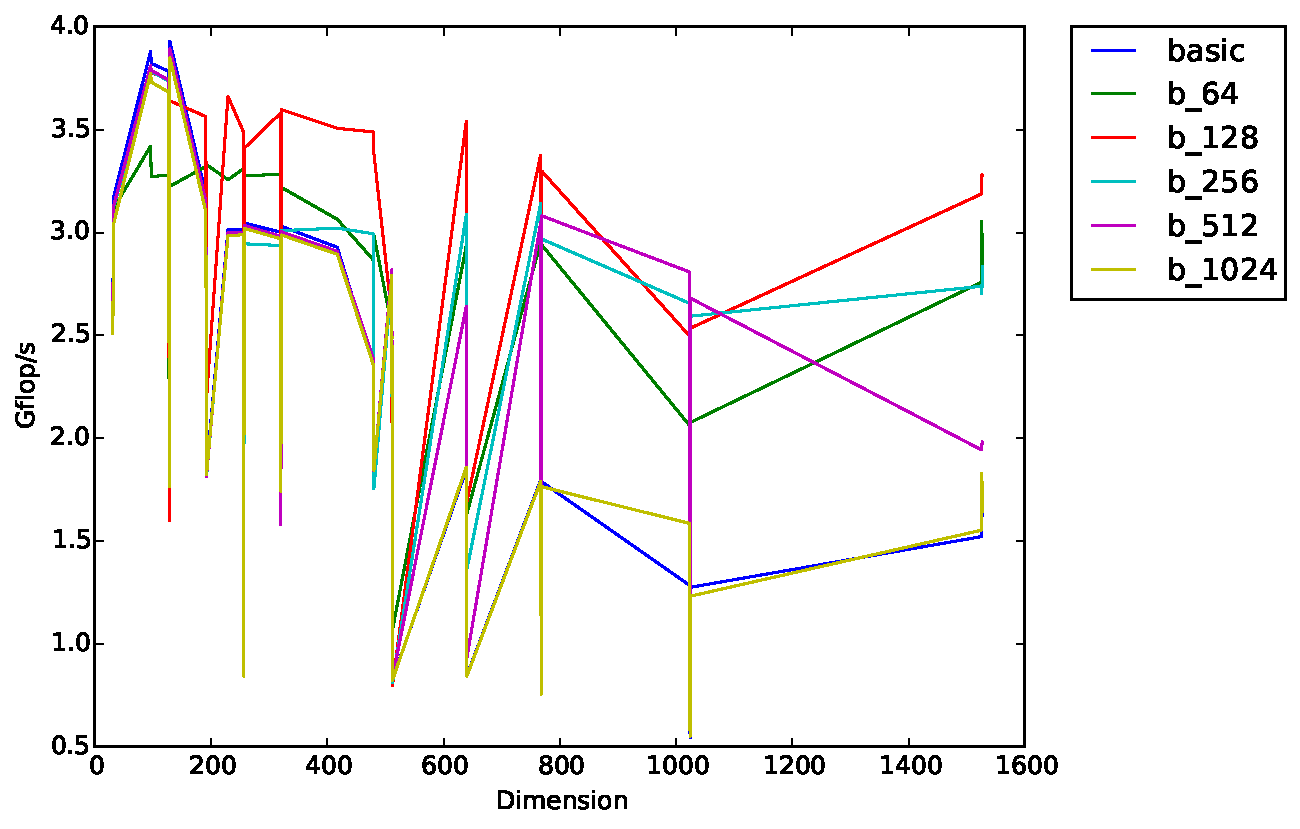
\includegraphics[width=0.85\textwidth] {timing_b_ijk_ijk_2}
        \end{center}
      \label{aload1}
      \caption{blocking with loop order $(i, j, k)\times(i, j, k)$}
  \end{subfigure}

\end{figure}

\subsection{Loop Order}

See Figure 3$-$7 below for loop order.
\\
The plot shows that looping performs the best with loop order $(j, k, i)$ for the basic implementation, as earlier hypothesized. Additionally, as expected, after matrix A is transposed, the loop order $(j,k,i)$ is no longer the most efficient.

\begin{figure}[!ht]
   \begin{subfigure}
      \centering
        \begin{center}
      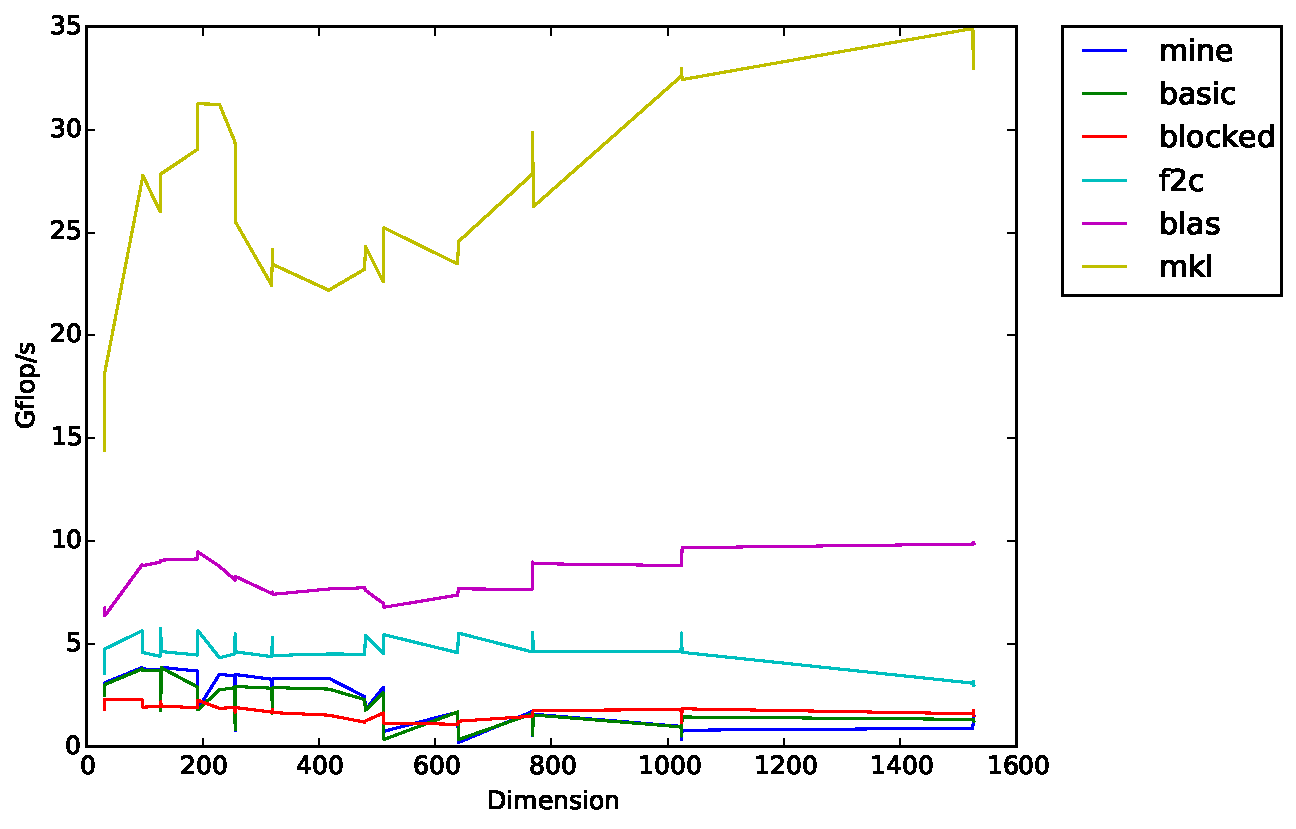
\includegraphics[width=0.85\textwidth] {ijk}
        \end{center}
      \label{aload0}
      \caption{loop order $(i, j, k)$}
  \end{subfigure}
  \begin{subfigure}
      \centering
        \begin{center}
      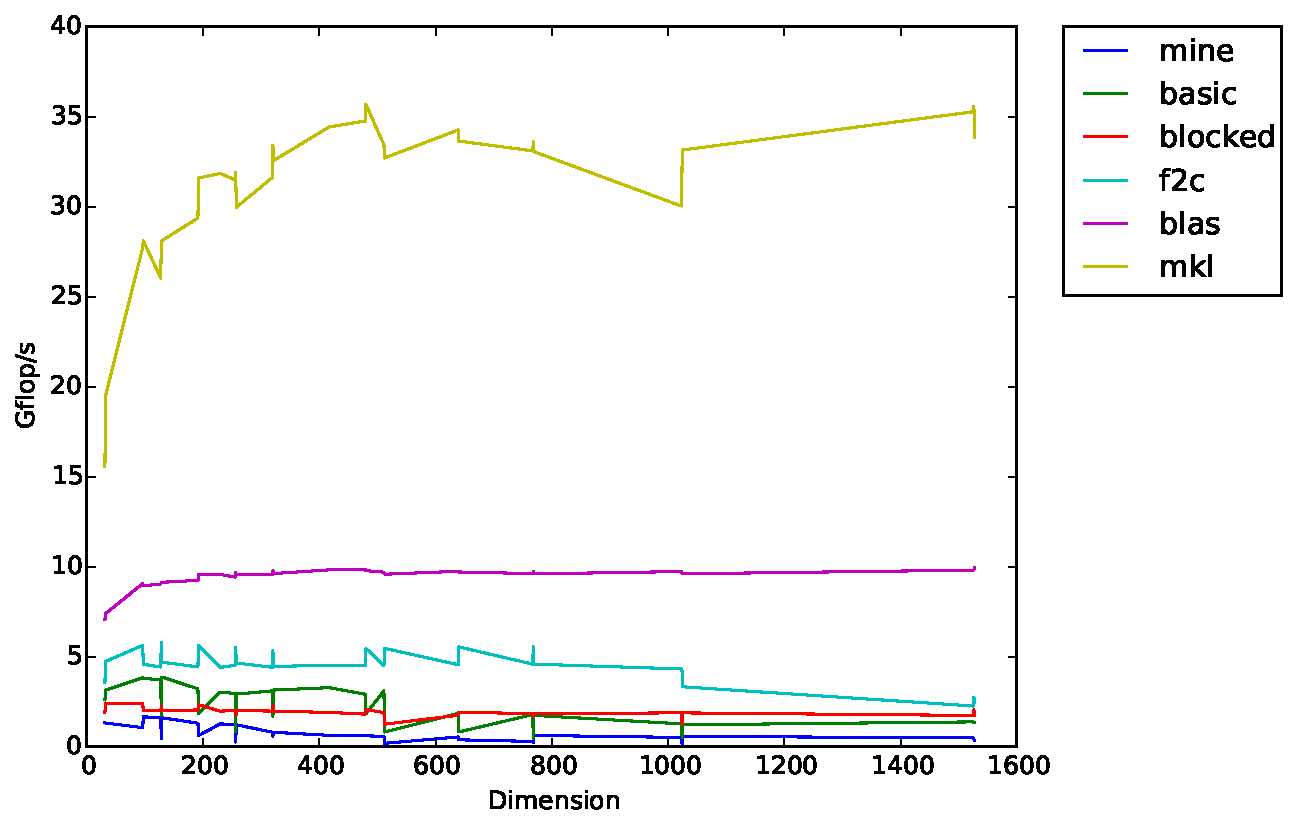
\includegraphics[width=0.85\textwidth] {ikj}
        \end{center}
      \label{aload1}
      \caption{loop order $(i, k, j)$}
  \end{subfigure}

\end{figure}

\begin{figure}[!ht]
   \begin{subfigure}
      \centering
        \begin{center}
      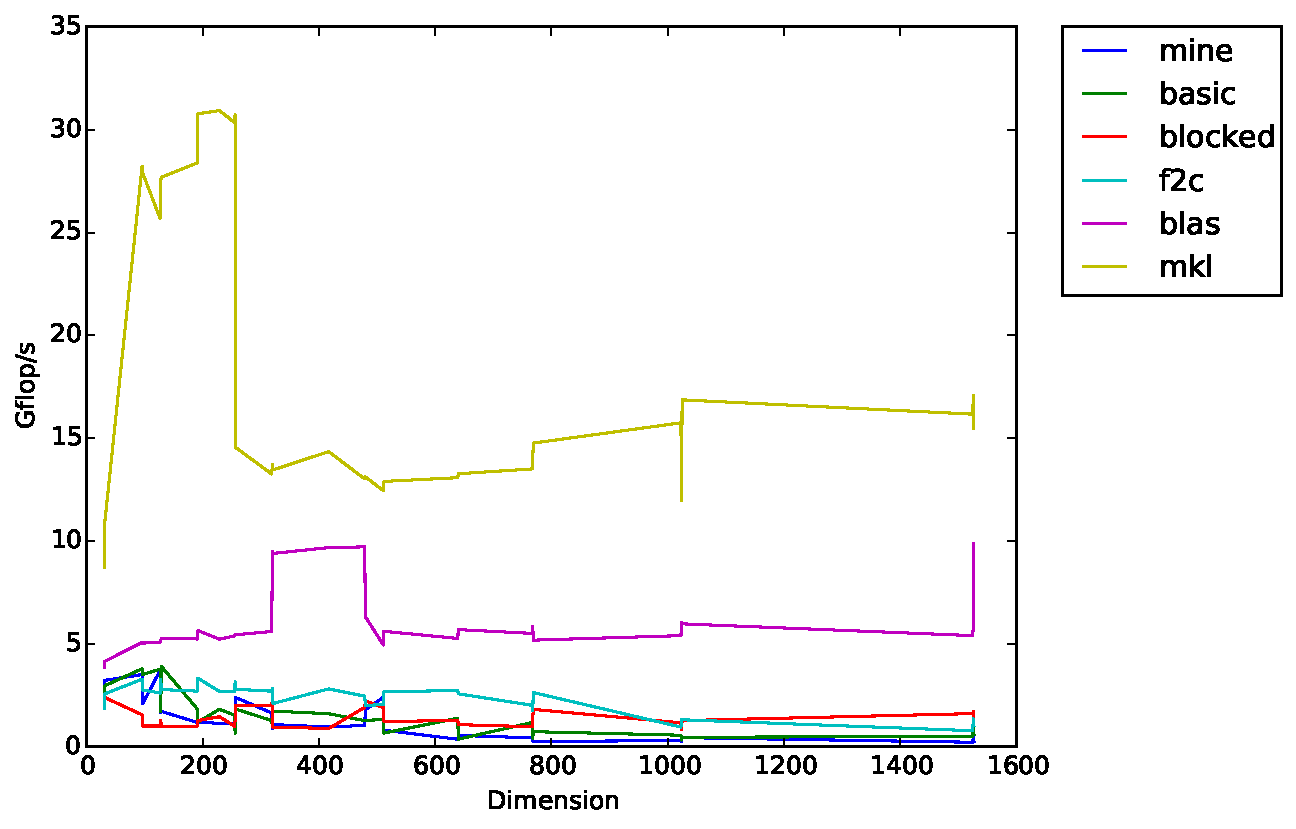
\includegraphics[width=0.85\textwidth] {jik}
        \end{center}
      \label{aload0}
      \caption{loop order $(j, i, k)$}
  \end{subfigure}
  \begin{subfigure}
      \centering
        \begin{center}
      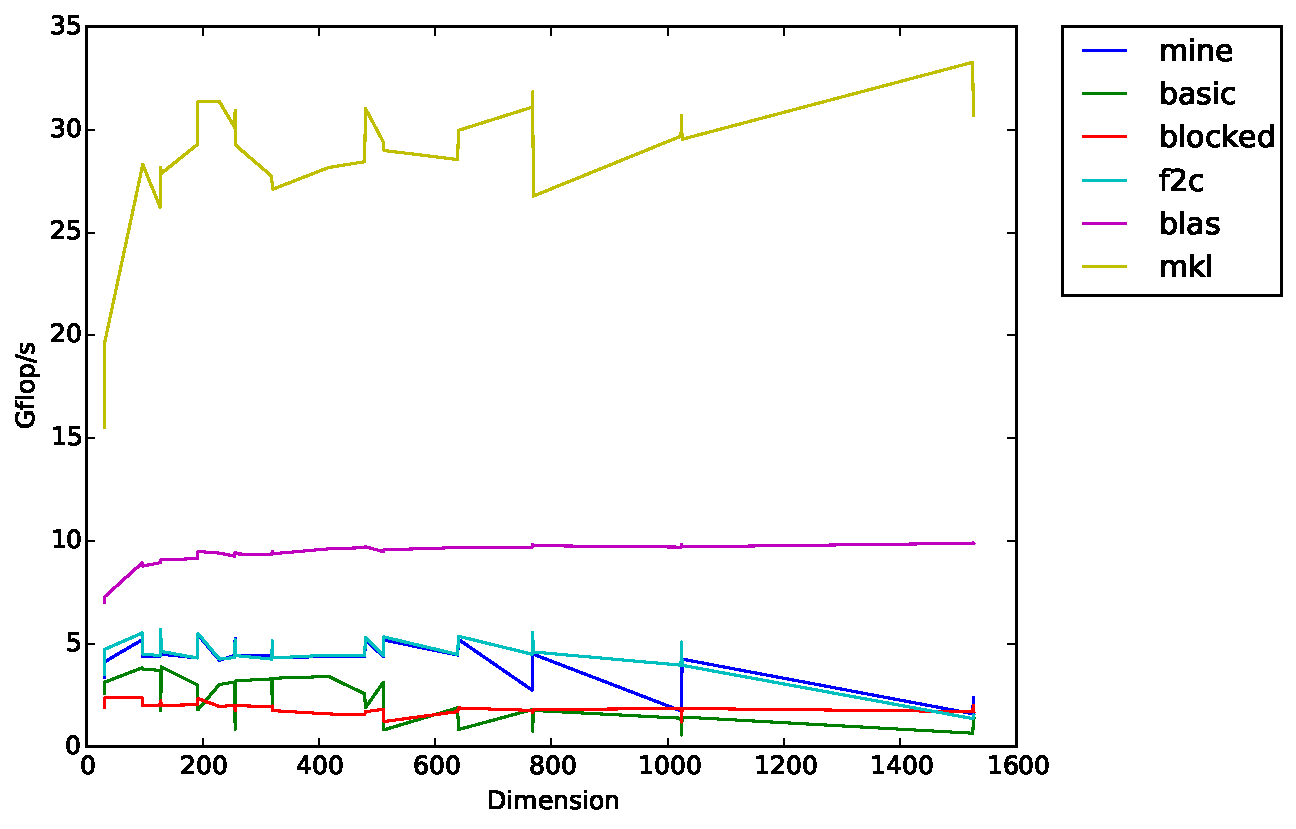
\includegraphics[width=0.85\textwidth] {jki}
        \end{center}
      \label{aload1}
      \caption{loop order $(j, k, i)$}
  \end{subfigure}

\end{figure}

\begin{figure}[!ht]
  \begin{subfigure}
    \centering
      \begin{center}
    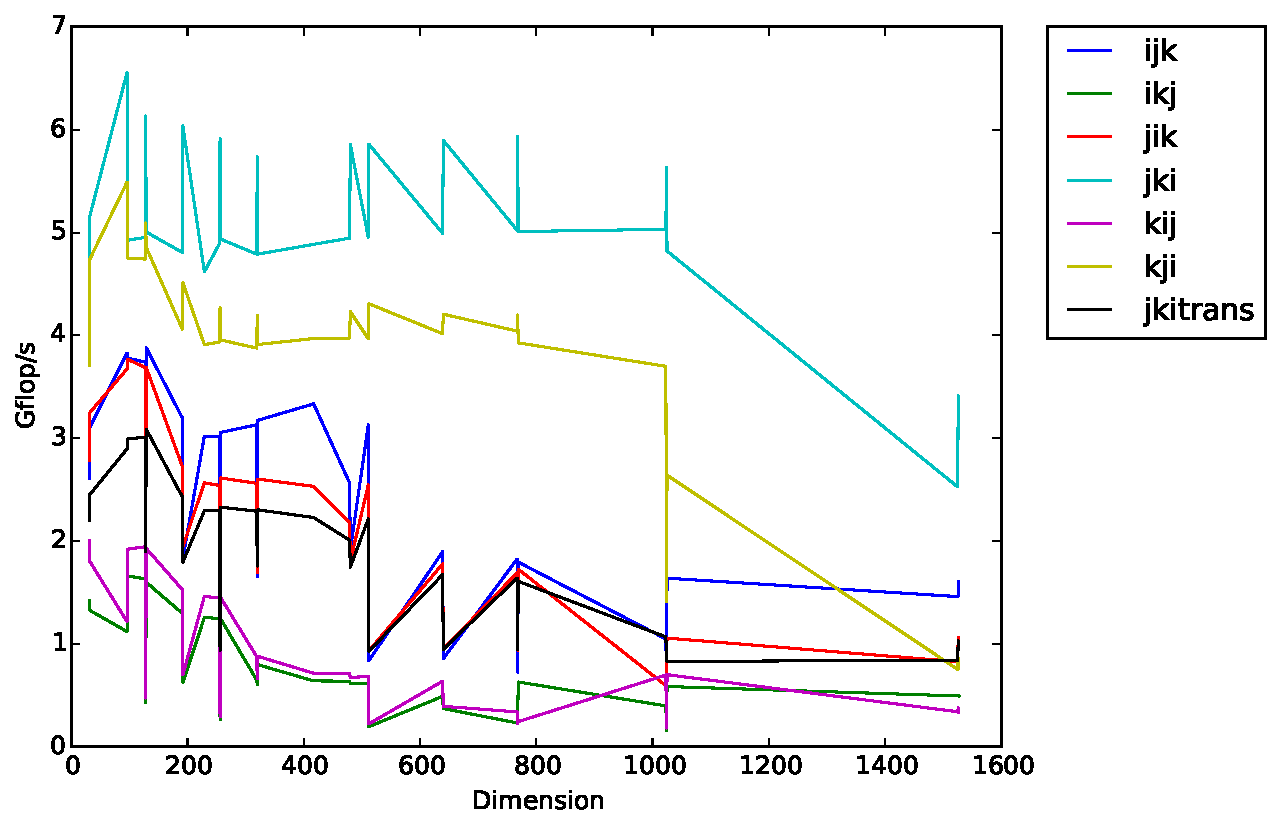
\includegraphics[width=0.85\textwidth] {timing_loops_trans}
      \end{center}
    \label{aload1}
    \caption{loop orders with transpose}
  \end{subfigure}

\end{figure}

\subsection{Blocking and Loop Order}

See Figure 8$-$13 below for blocking with loop order.
\\
The plot shows that blocking and looping performs the best with block size $256, 512$ and loop order $(i, j, k)\times(j, k, i), (j, k, i)\times(j, k, i)$.

\begin{figure}[!ht]
   \begin{subfigure}
      \centering
        \begin{center}
      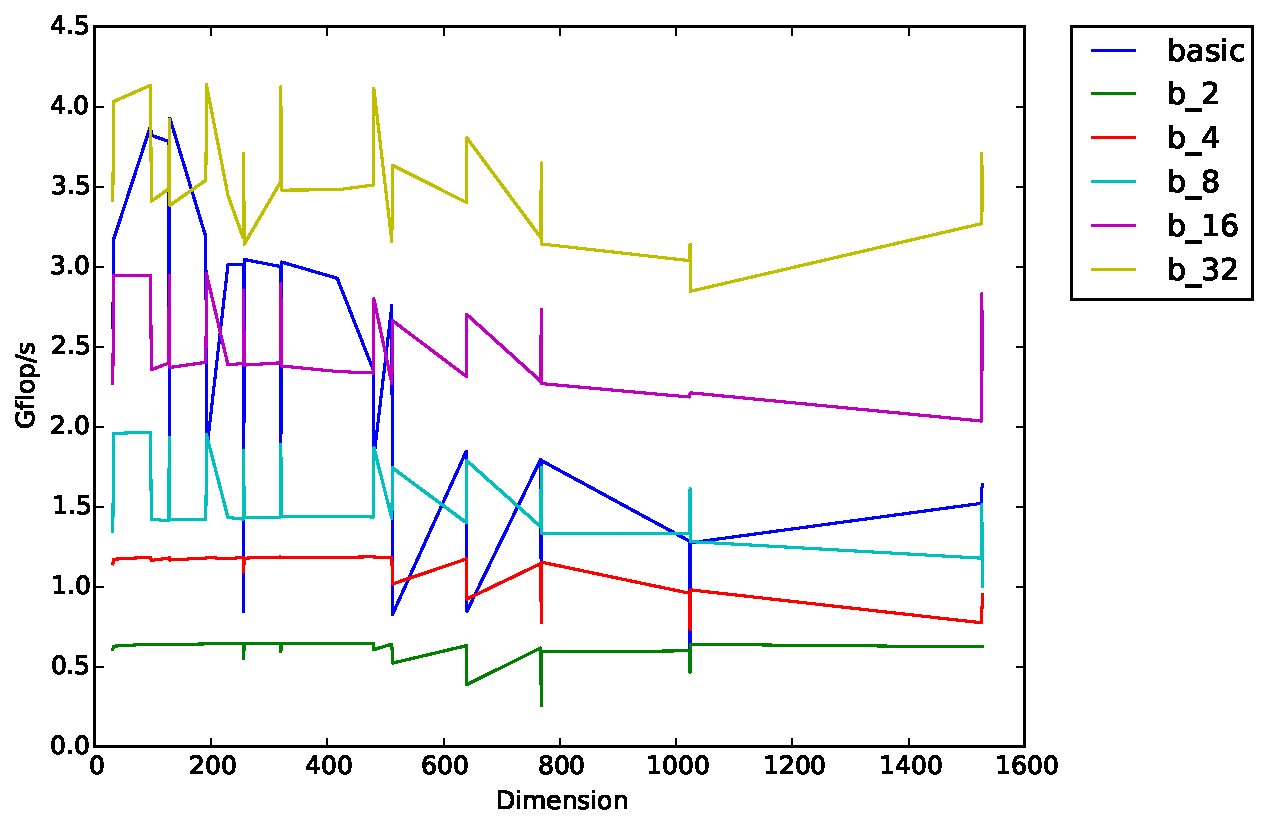
\includegraphics[width=0.85\textwidth] {timing_b_ijk_jki_1}
        \end{center}
      \label{aload0}
      \caption{blocking with loop order $(i, j, k)\times(j, k, i)$}
  \end{subfigure}
  \begin{subfigure}
      \centering
        \begin{center}
      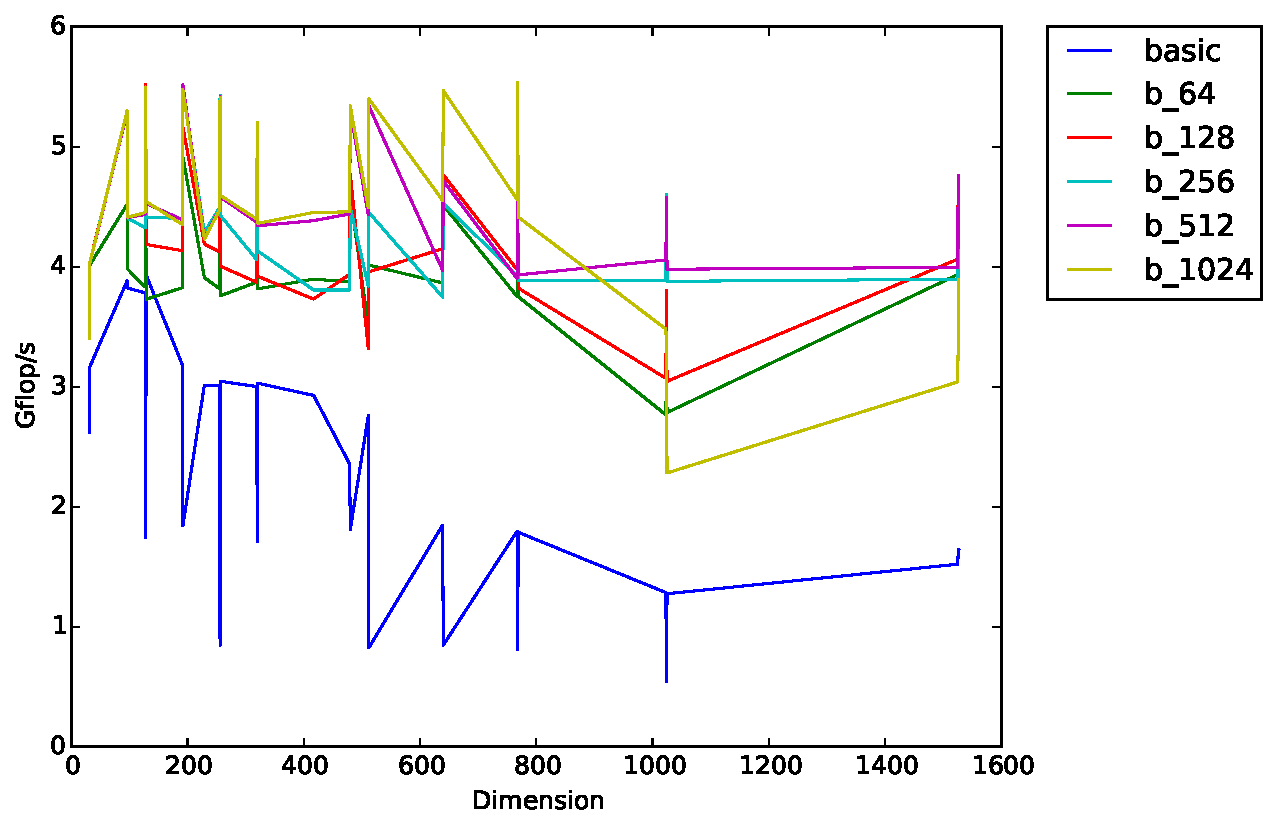
\includegraphics[width=0.85\textwidth] {timing_b_ijk_jki_2}
        \end{center}
      \label{aload1}
      \caption{blocking with loop order $(i, j, k)\times(j, k, i)$}
  \end{subfigure}

\end{figure}

\begin{figure}[!ht]
   \begin{subfigure}
      \centering
        \begin{center}
      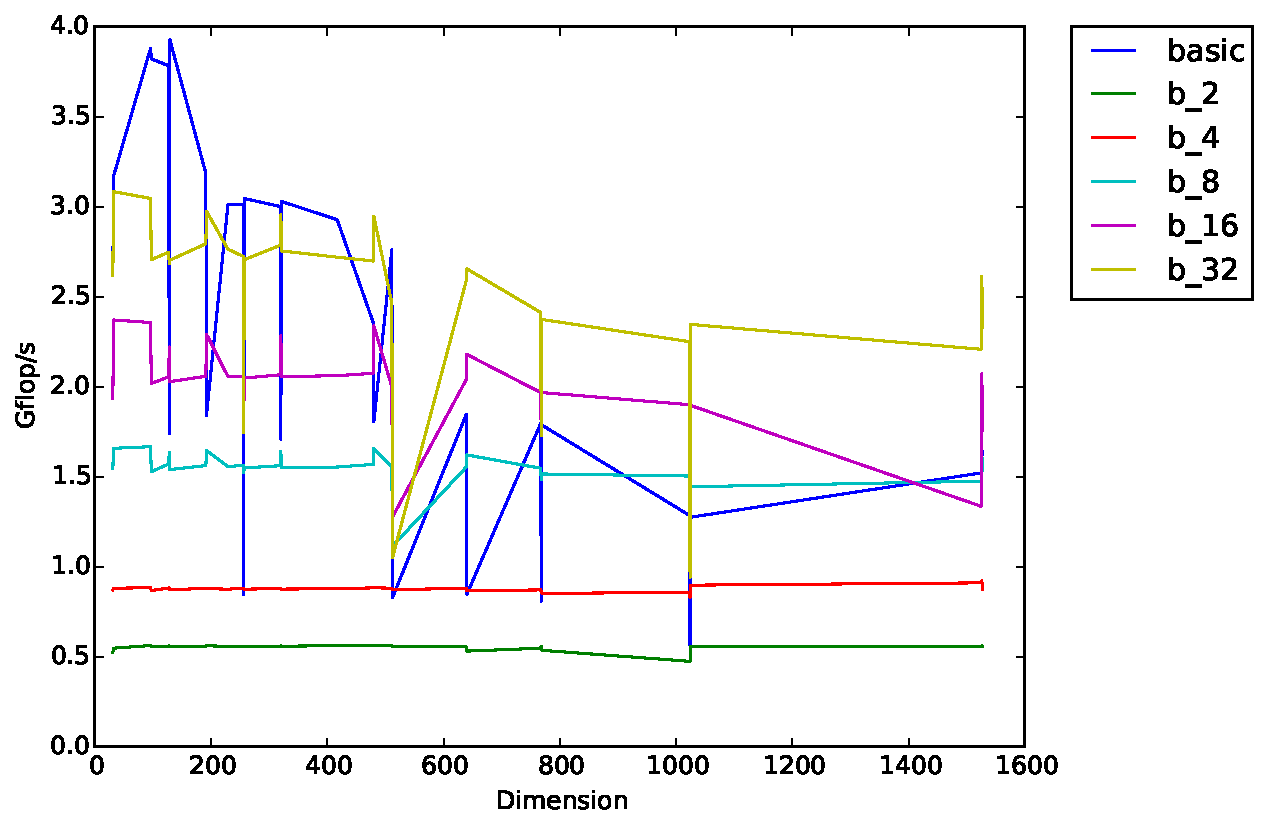
\includegraphics[width=0.85\textwidth] {timing_b_jki_ijk_1}
        \end{center}
      \label{aload0}
      \caption{blocking with loop order $(j, k, i)\times(i, j, k)$}
  \end{subfigure}
  \begin{subfigure}
      \centering
        \begin{center}
      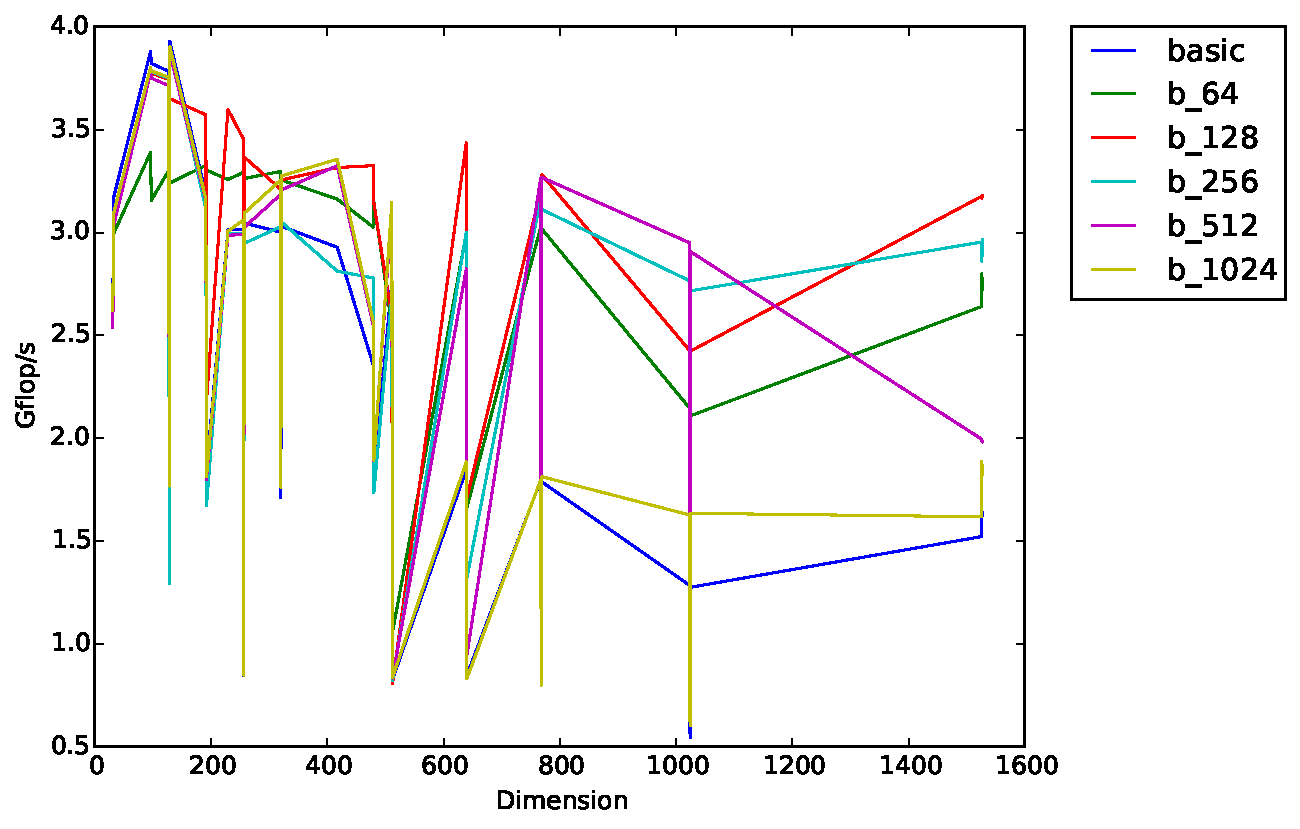
\includegraphics[width=0.85\textwidth] {timing_b_jki_ijk_2}
        \end{center}
      \label{aload1}
      \caption{blocking with loop order $(j, k, i)\times(i, j, k)$}
  \end{subfigure}

\end{figure}

\begin{figure}[!ht]
   \begin{subfigure}
      \centering
        \begin{center}
      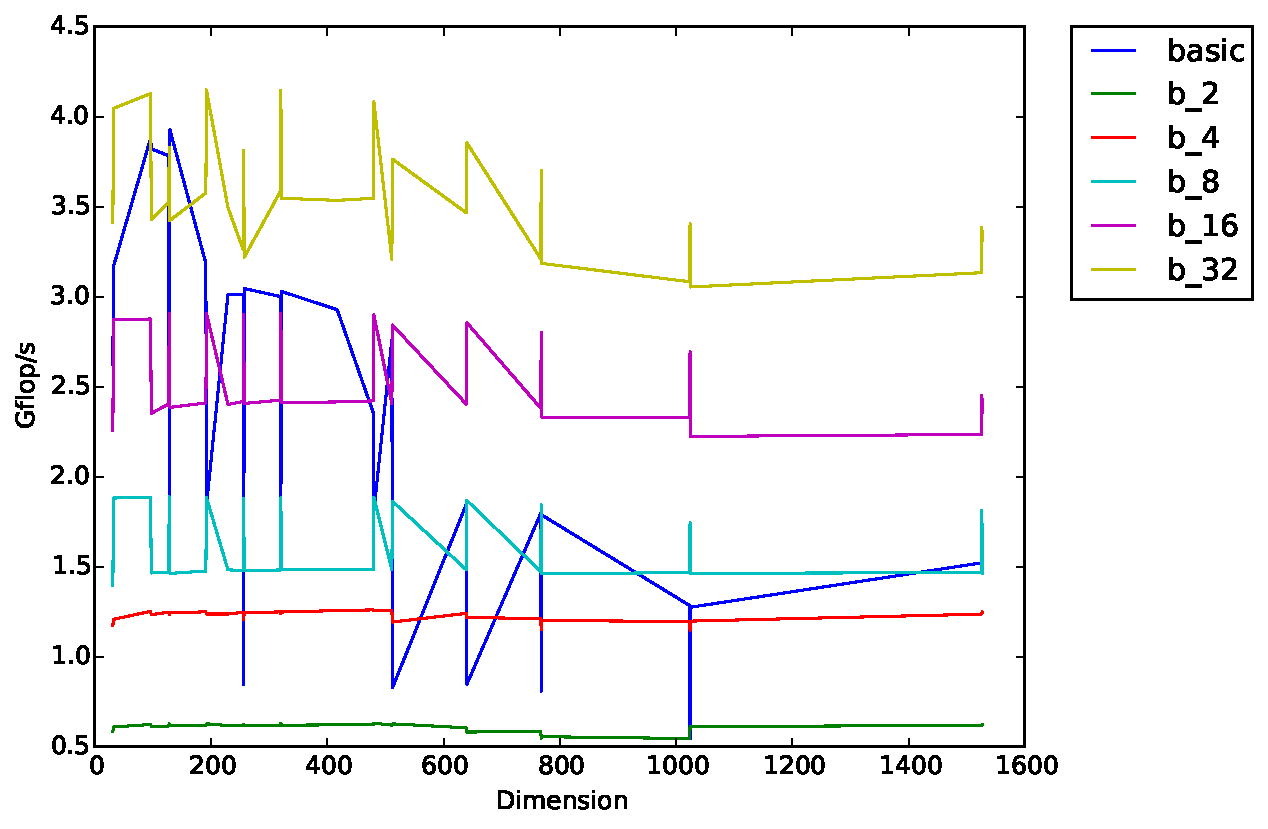
\includegraphics[width=0.85\textwidth] {timing_b_jki_jki_1}
        \end{center}
      \label{aload0}
      \caption{blocking with loop order $(j, k, i)\times(j, k, i)$}
  \end{subfigure}
  \begin{subfigure}
      \centering
        \begin{center}
      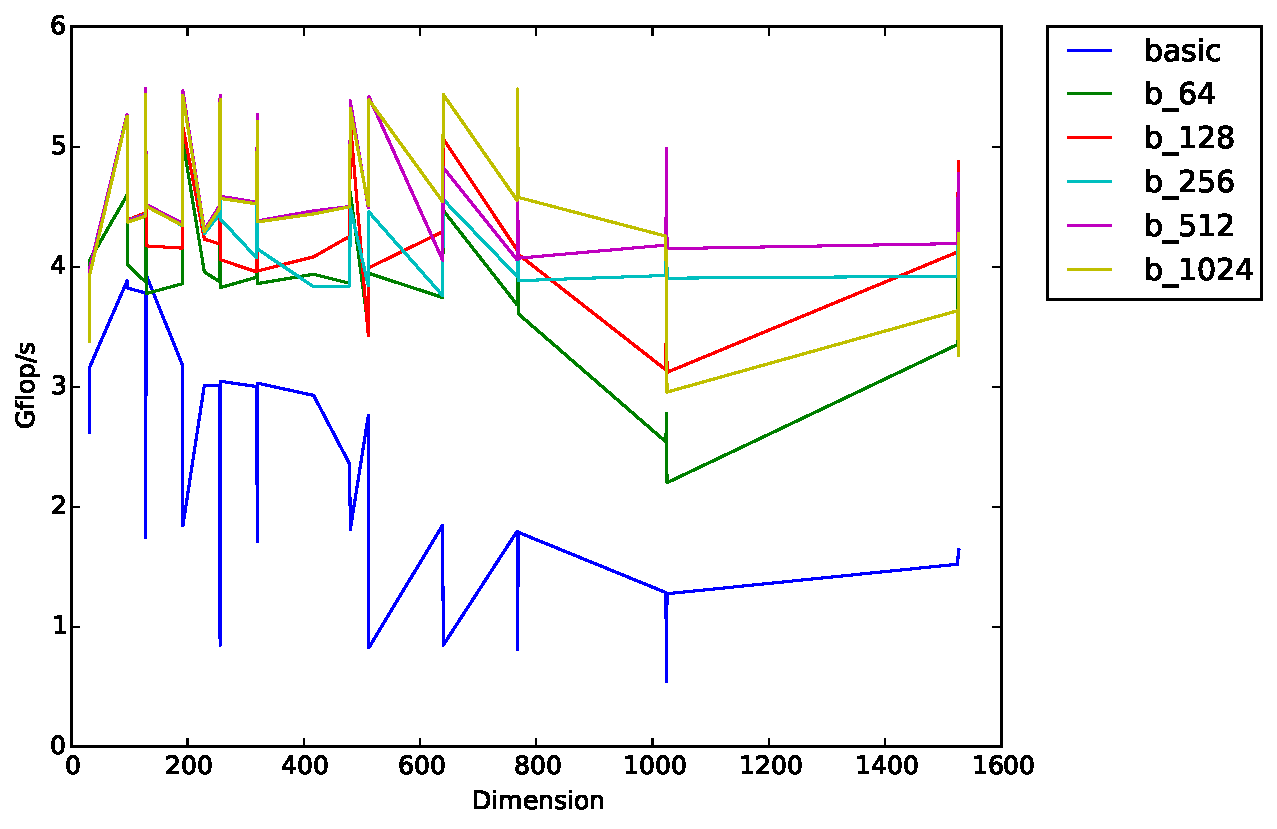
\includegraphics[width=0.85\textwidth] {timing_b_jki_jki_2}
        \end{center}
      \label{aload1}
      \caption{blocking with loop order $(j, k, i)\times(j, k, i)$}
  \end{subfigure}

\end{figure}





\subsection{Blocking and Copy Optimization}

See Figure 14 and 15 below for blocking with default loop order $(i, j, k)\times(i, j, k)$ and copy optimization.
\\
The plot shows that blocking and copying performs the best with block size $8, 128, 512$.

\begin{figure}[!ht]
   \begin{subfigure}
      \centering
        \begin{center}
      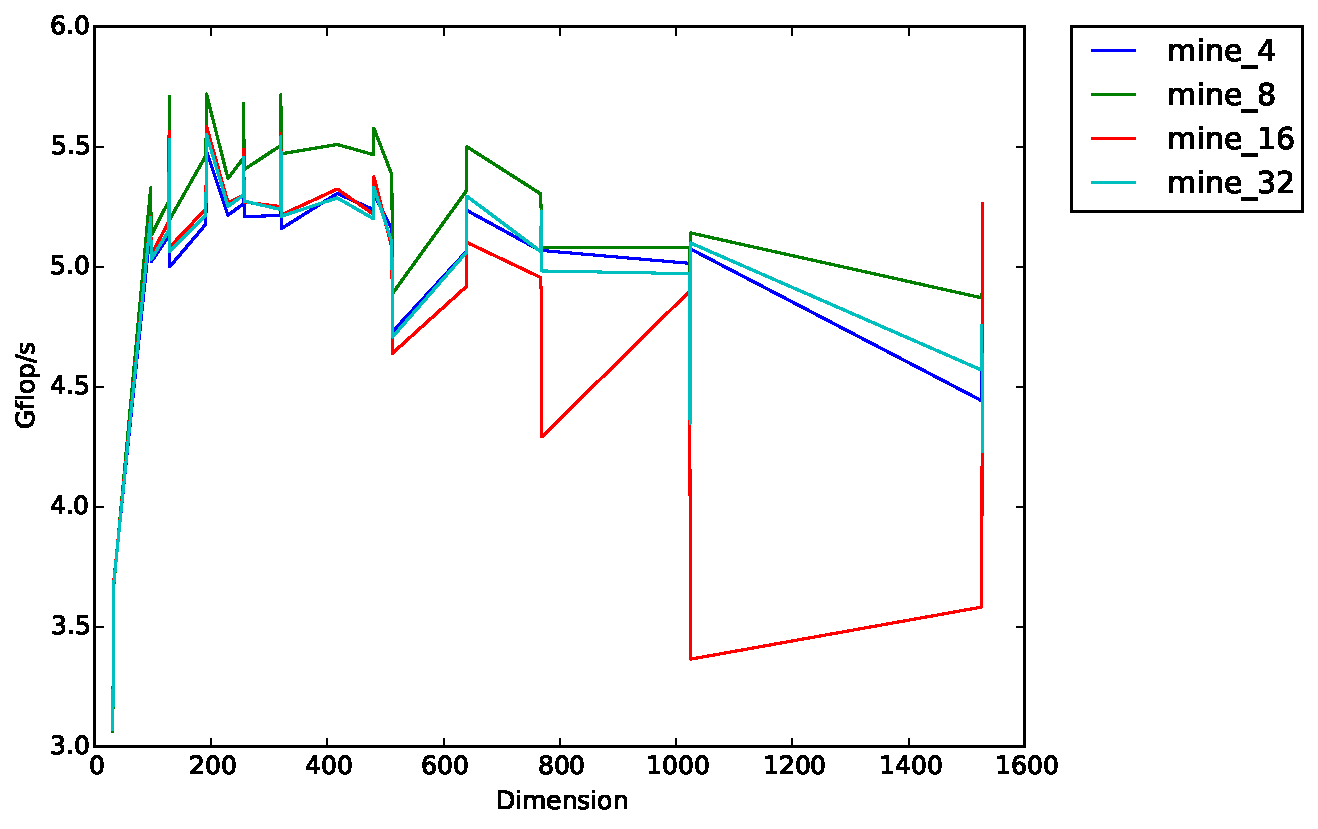
\includegraphics[width=0.85\textwidth] {timing_ijk_ijk_1}
        \end{center}
      \label{aload0}
      \caption{blocking with loop order $(i, j, k)\times(i, j, k)$ and copy optimization}
  \end{subfigure}
  \begin{subfigure}
      \centering
        \begin{center}
      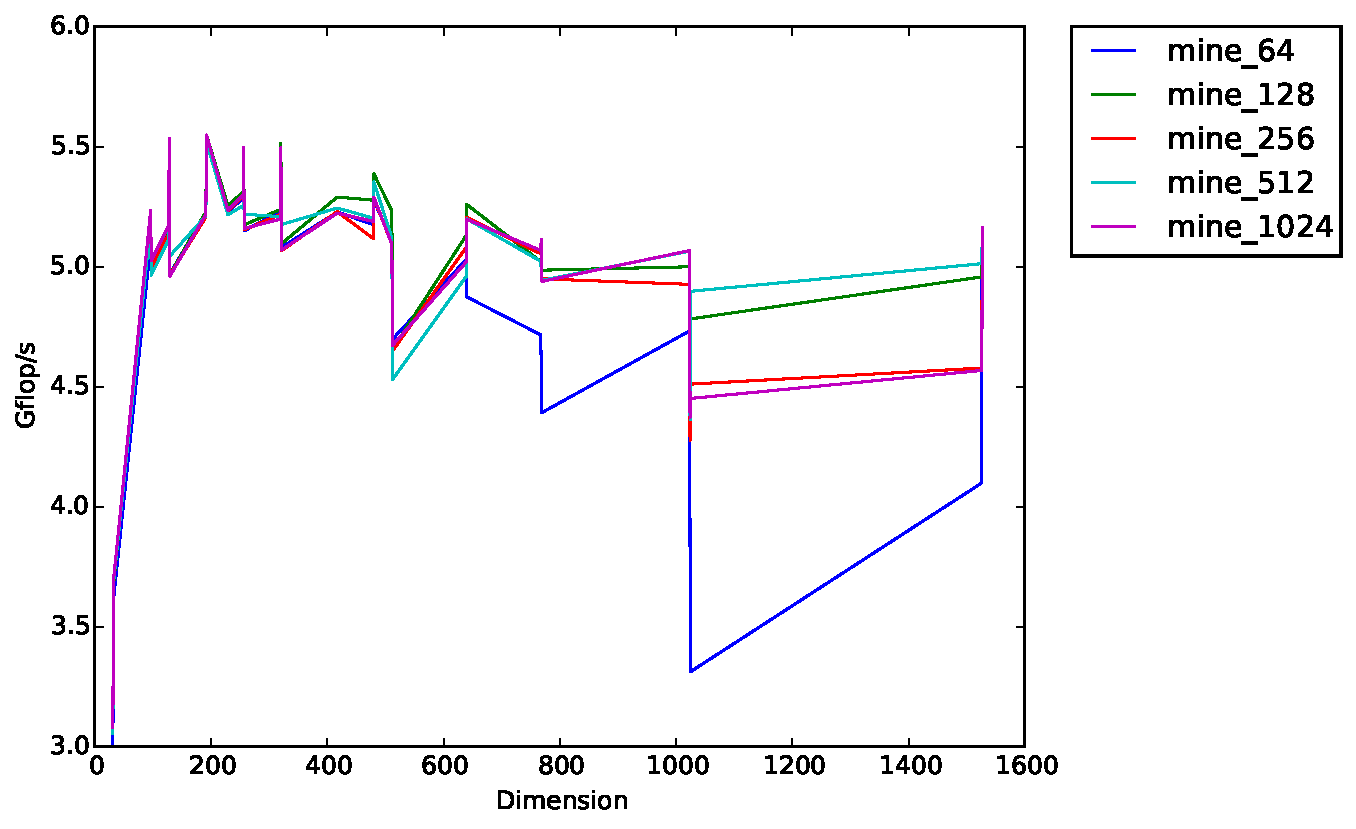
\includegraphics[width=0.85\textwidth] {timing_ijk_ijk_2}
        \end{center}
      \label{aload1}
      \caption{blocking with loop order $(i, j, k)\times(i, j, k)$ and copy optimization}
  \end{subfigure}

\end{figure}

\subsection{Blocking, Loop Order and Copy Optimization}

See Figure 16$-$21 below for blocking with loop order and copy optimization.
\\
The plot shows that blocking, looping and copying performs the best with block size $16, 32$ and loop order $(i, j, k)\times(j, i, k)$.

\begin{figure}[!ht]
   \begin{subfigure}
      \centering
        \begin{center}
      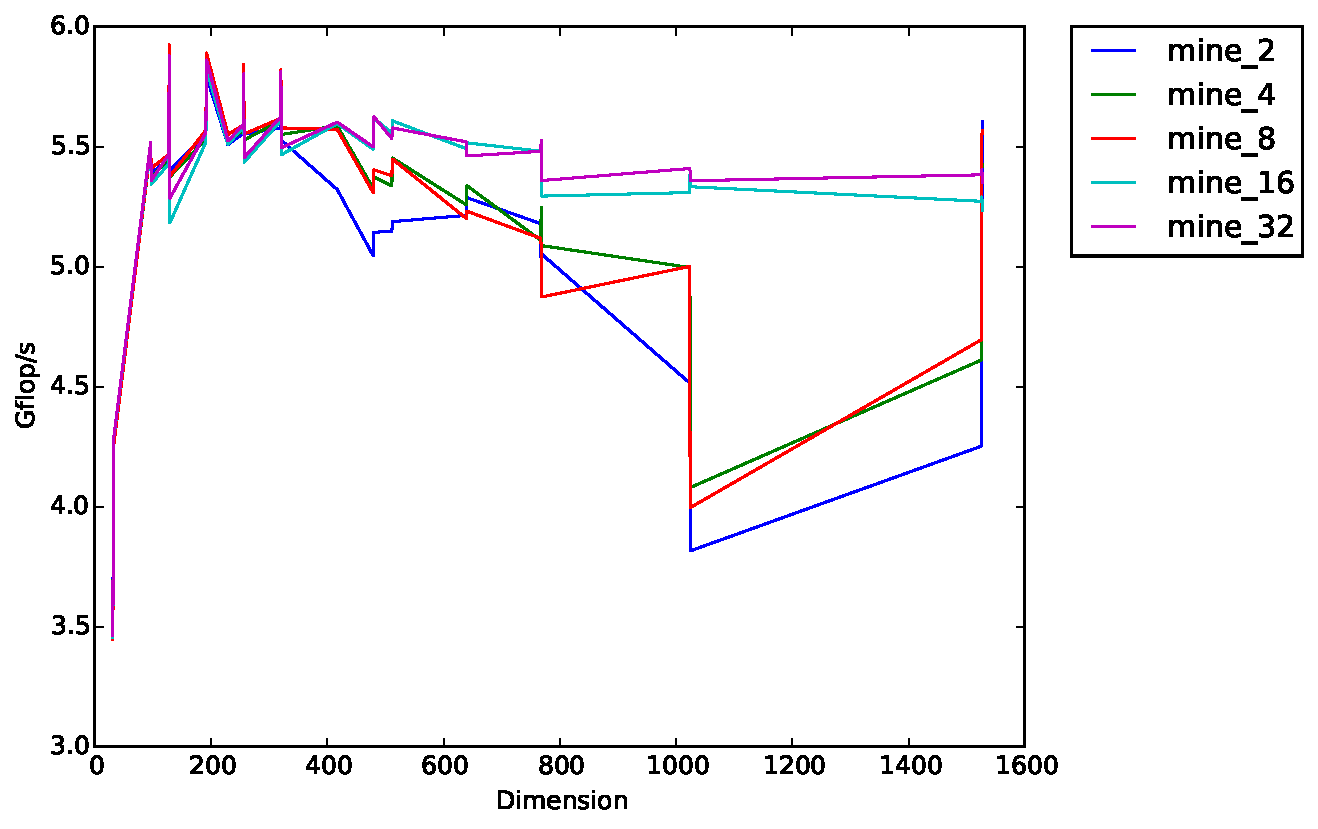
\includegraphics[width=0.85\textwidth] {timing_ijk_jik_1}
        \end{center}
      \label{aload0}
      \caption{blocking with loop order $(i, j, k)\times(j, i, k)$ and copy optimization}
  \end{subfigure}
  \begin{subfigure}
      \centering
        \begin{center}
      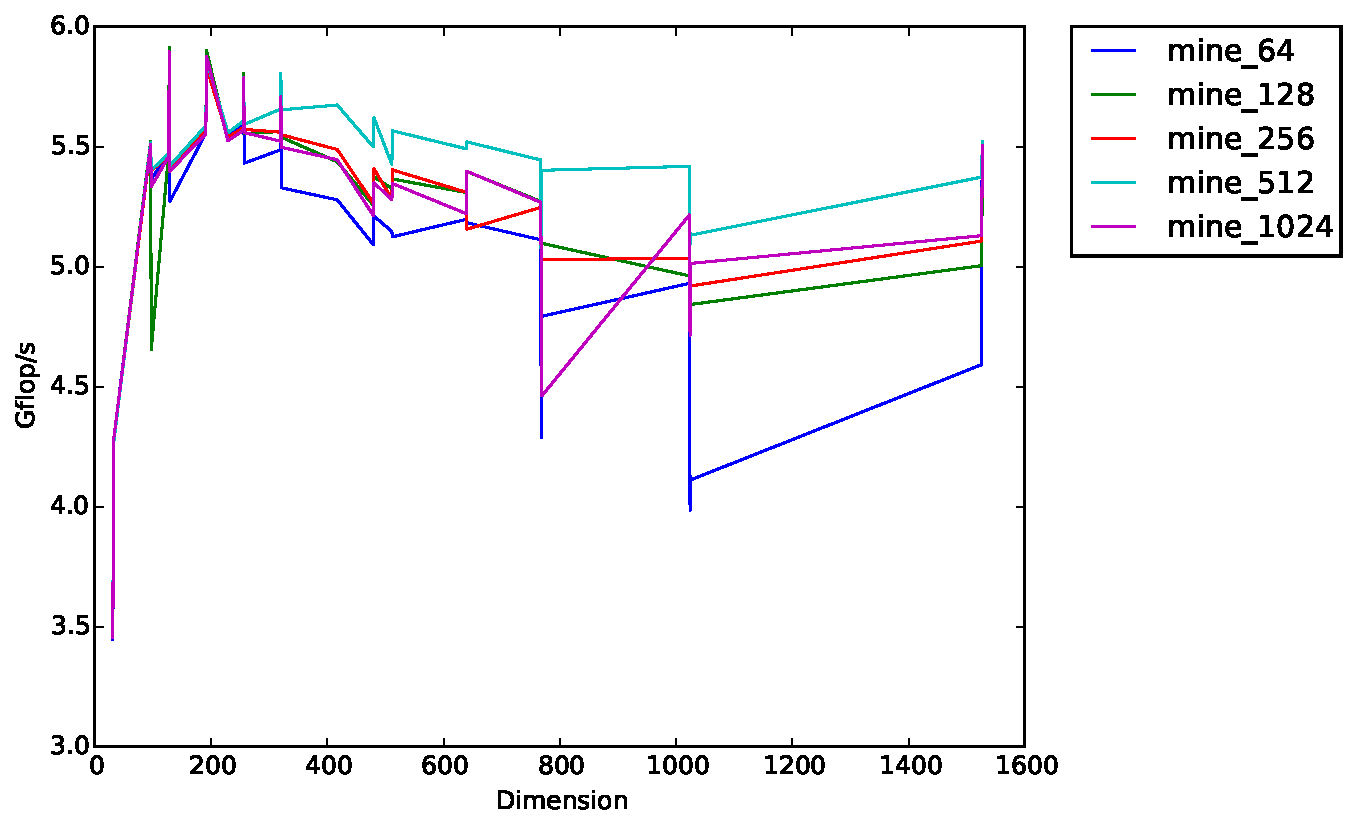
\includegraphics[width=0.85\textwidth] {timing_ijk_jik_2}
        \end{center}
      \label{aload1}
      \caption{blocking with loop order $(i, j, k)\times(j, i, k)$ and copy optimization}
  \end{subfigure}

\end{figure}

\begin{figure}[!ht]
   \begin{subfigure}
      \centering
        \begin{center}
      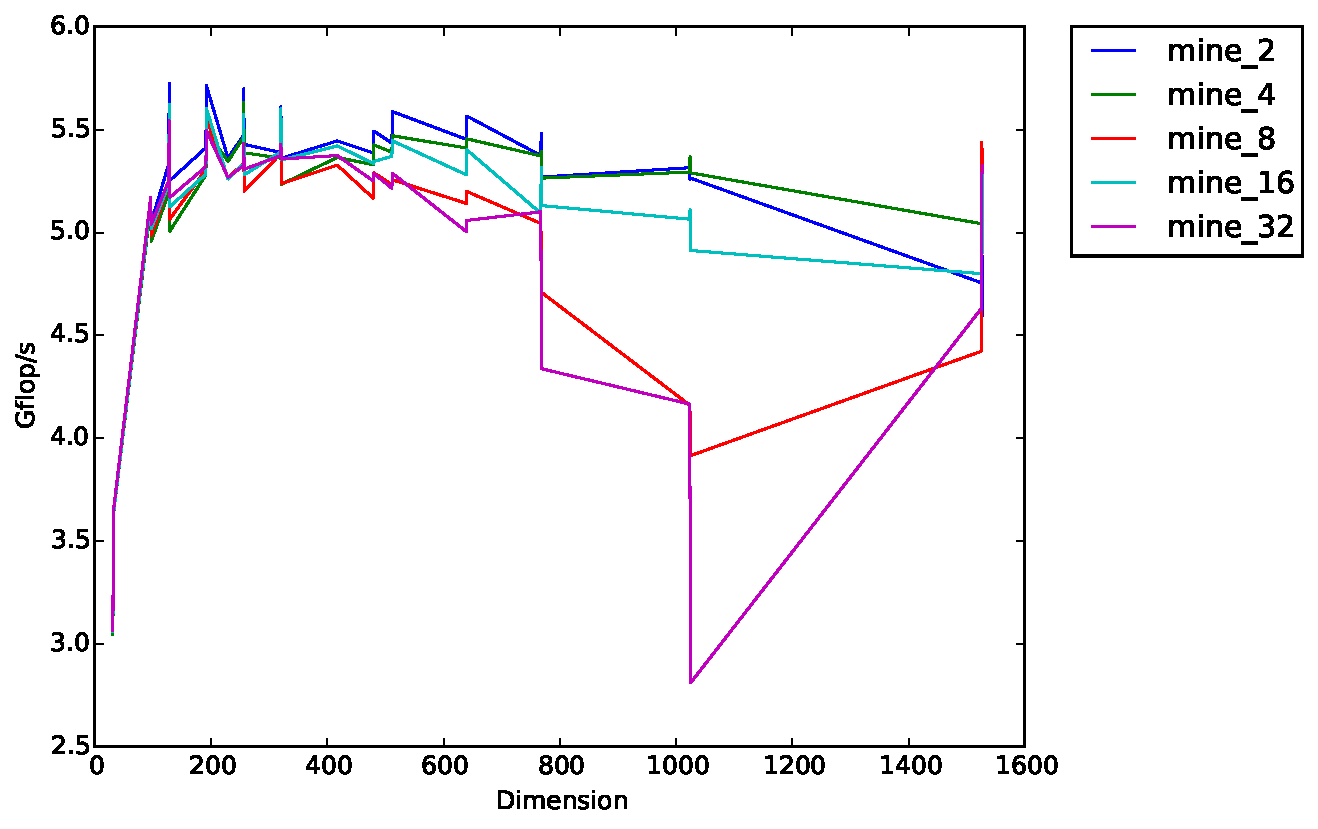
\includegraphics[width=0.85\textwidth] {timing_jik_jik_1}
        \end{center}
      \label{aload0}
      \caption{blocking with loop order $(j, i, k)\times(j, i, k)$ and copy optimization}
  \end{subfigure}
  \begin{subfigure}
      \centering
        \begin{center}
      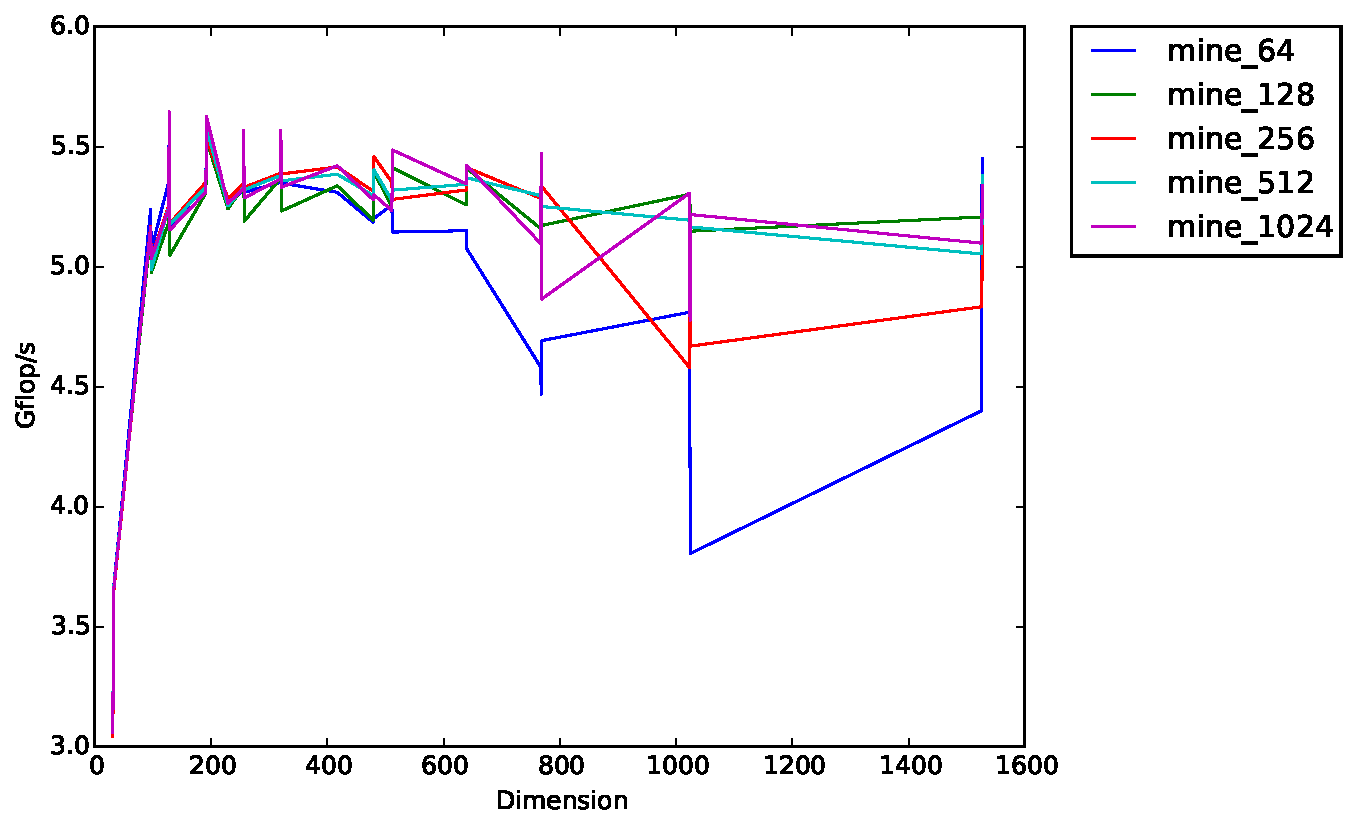
\includegraphics[width=0.85\textwidth] {timing_jik_jik_2}
        \end{center}
      \label{aload1}
      \caption{blocking with loop order $(j, i, k)\times(j, i, k)$ and copy optimization}
  \end{subfigure}

\end{figure}

\begin{figure}[!ht]
   \begin{subfigure}
      \centering
        \begin{center}
      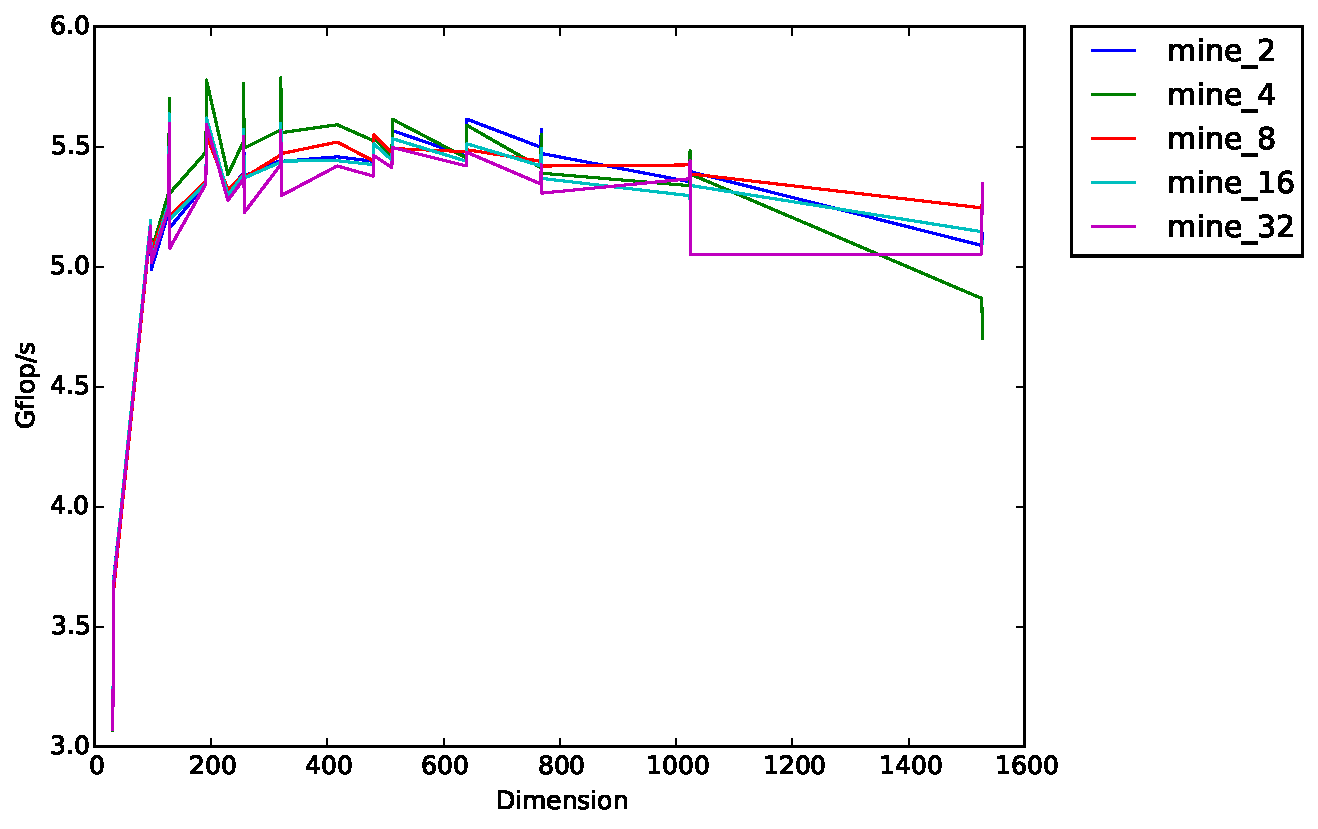
\includegraphics[width=0.85\textwidth] {timing_jki_jik_1}
        \end{center}
      \label{aload0}
      \caption{blocking with loop order $(j, k, i)\times(j, i, k)$ and copy optimization}
  \end{subfigure}
  \begin{subfigure}
      \centering
        \begin{center}
      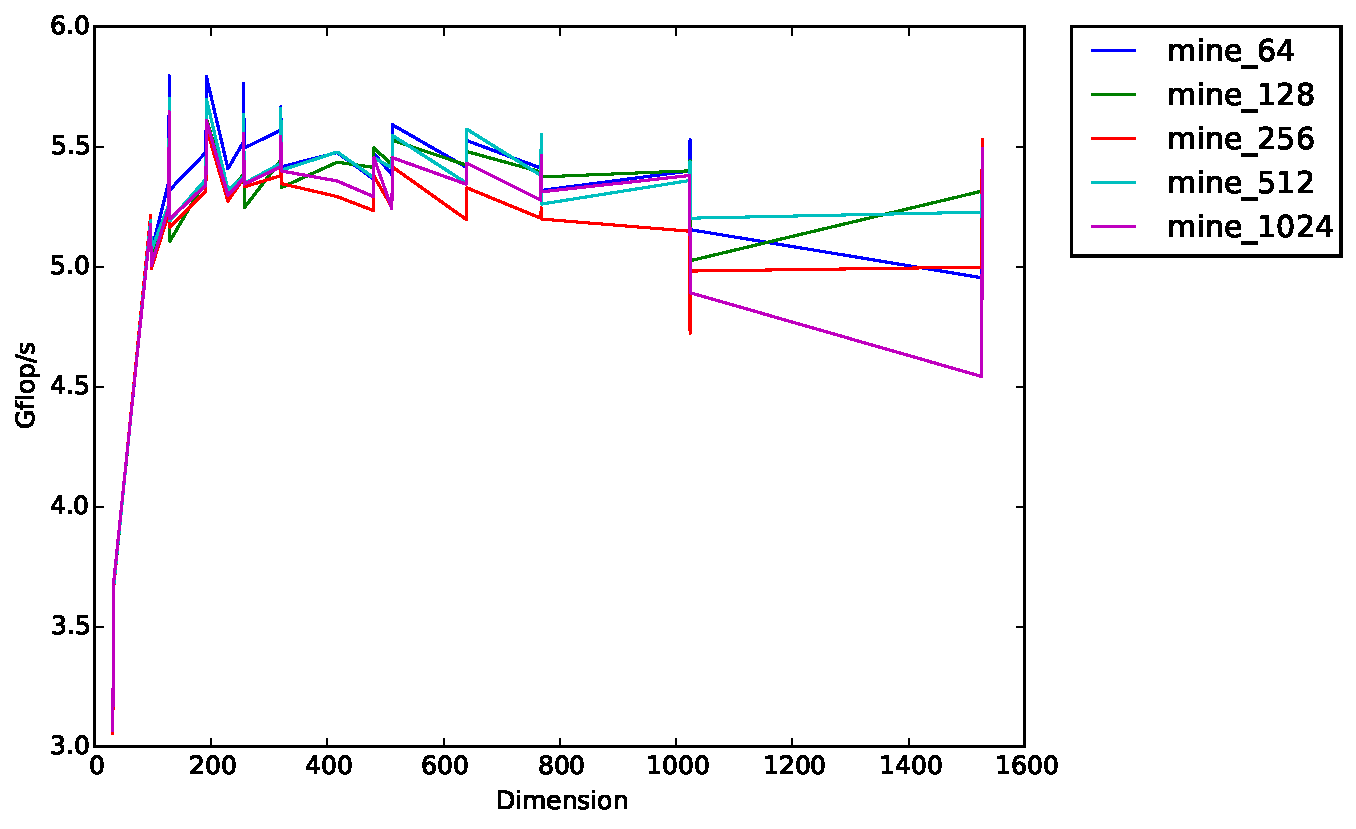
\includegraphics[width=0.85\textwidth] {timing_jki_jik_2}
        \end{center}
      \label{aload1}
      \caption{blocking with loop order $(j, k, i)\times(j, i, k)$ and copy optimization}
  \end{subfigure}

\end{figure}





\subsection{Compiler Flag}

See Figure 22 below for unrolling loops in compiler flags.
\\
The plot shows that unrolling loops in compiler flags alone does not make much difference.

\begin{figure}[!ht]
\begin{center}
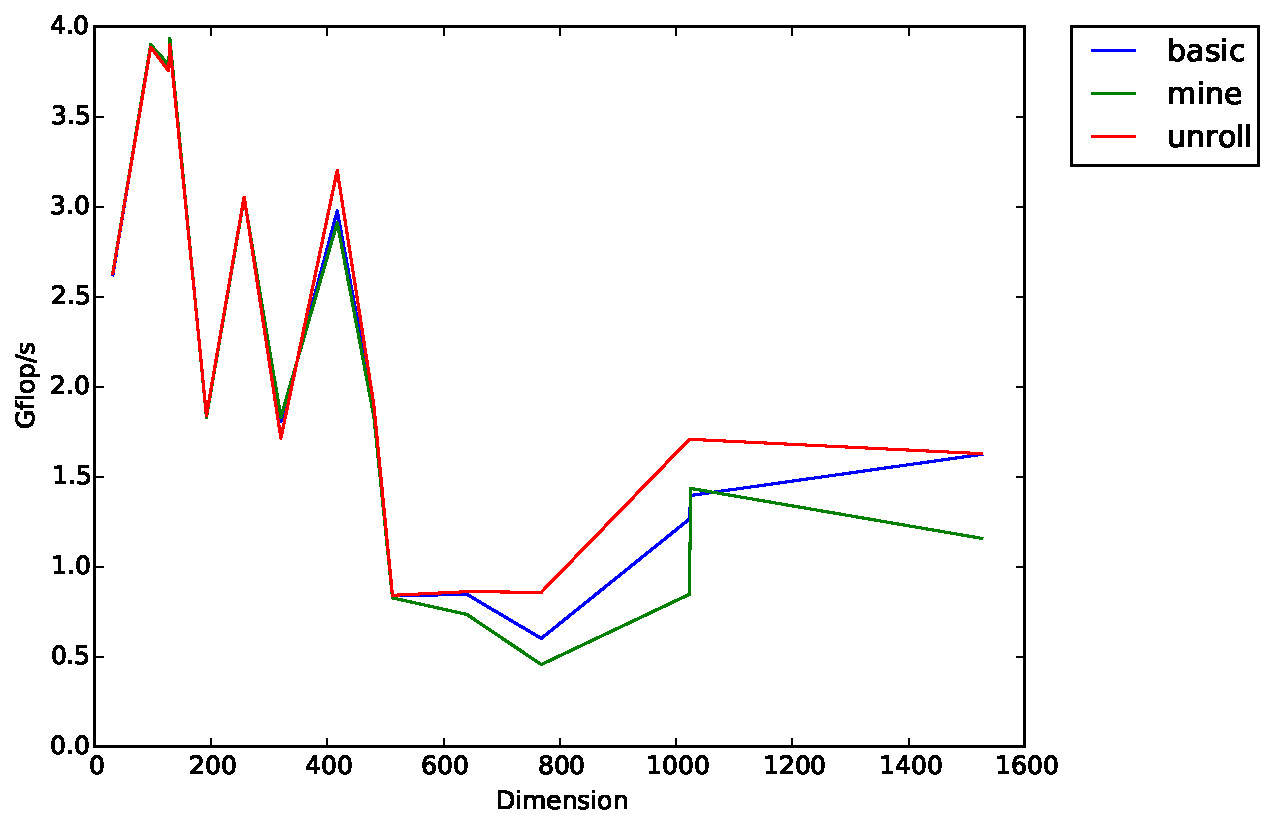
\includegraphics[width=0.85\textwidth] {timing_unroll}
\caption{unrolling loops in compiler flags}
\end{center}
\end{figure}




\section{Conclusion}

We summarize our finds and select the best method we have tried so far.

\subsection{Best Method}

The best algorithm we have tried so far is blocking, looping and copying with block size $16$ and loop order $(i, j, k)\times(j, i, k)$.
\\
Therefore, we carry out a local search around block size 16.
\\
See Figure 23$-$26 below for blocking with loop order and copy optimization.
\\
The plot shows that blocking, looping and copying performs the best with block size $8$ and loop order $(i, j, k)\times(j, i, k)$.
\\
Moreover, the performance of blocking, looping and copying is bad when size is less than 100. Thus, we combine a naive implementation with looping order $(j, k, i)$ with the blocking one.

\begin{figure}[!ht]
   \begin{subfigure}
      \centering
        \begin{center}
      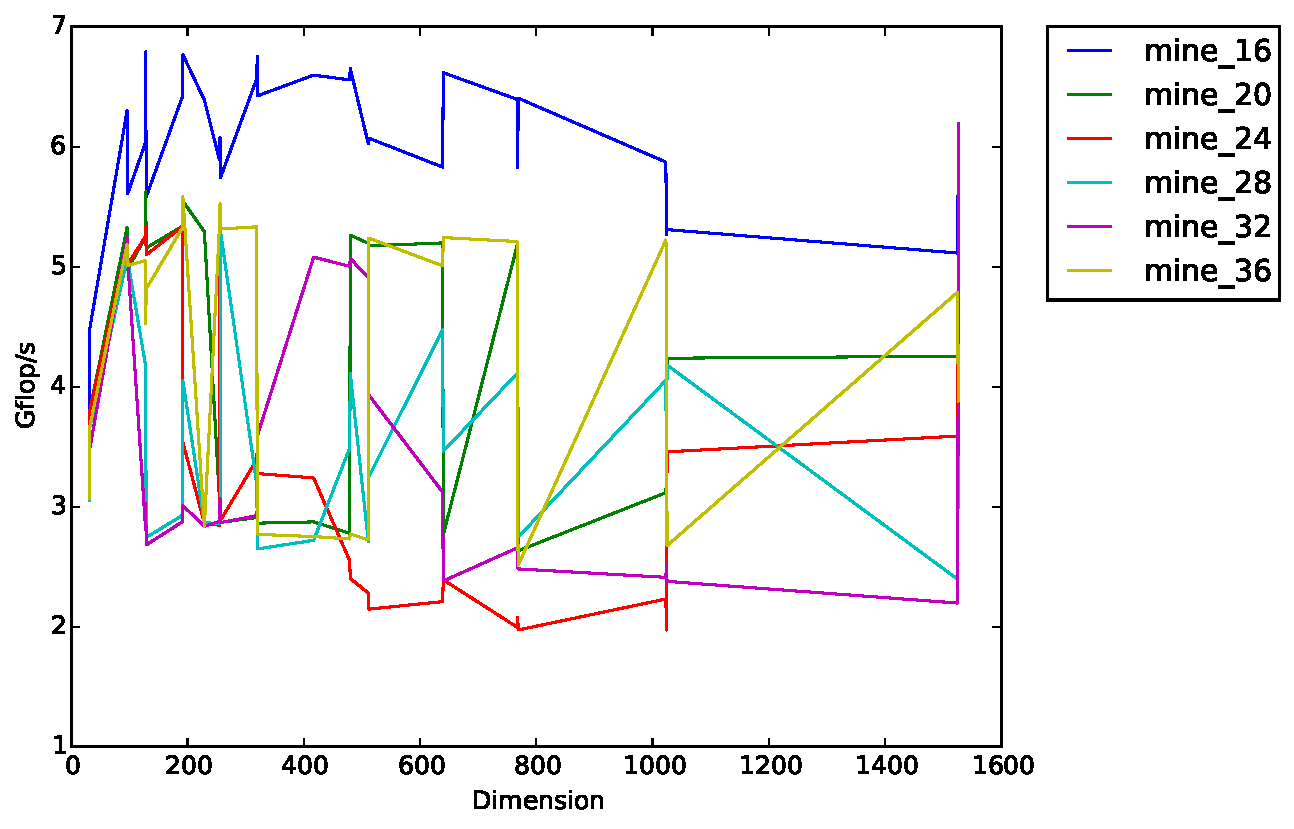
\includegraphics[width=0.85\textwidth] {timing_ijk_jik_3}
        \end{center}
      \label{aload0}
      \caption{blocking with loop order $(i, j, k)\times(j, i, k)$ and copy optimization}
  \end{subfigure}
  \begin{subfigure}
      \centering
        \begin{center}
      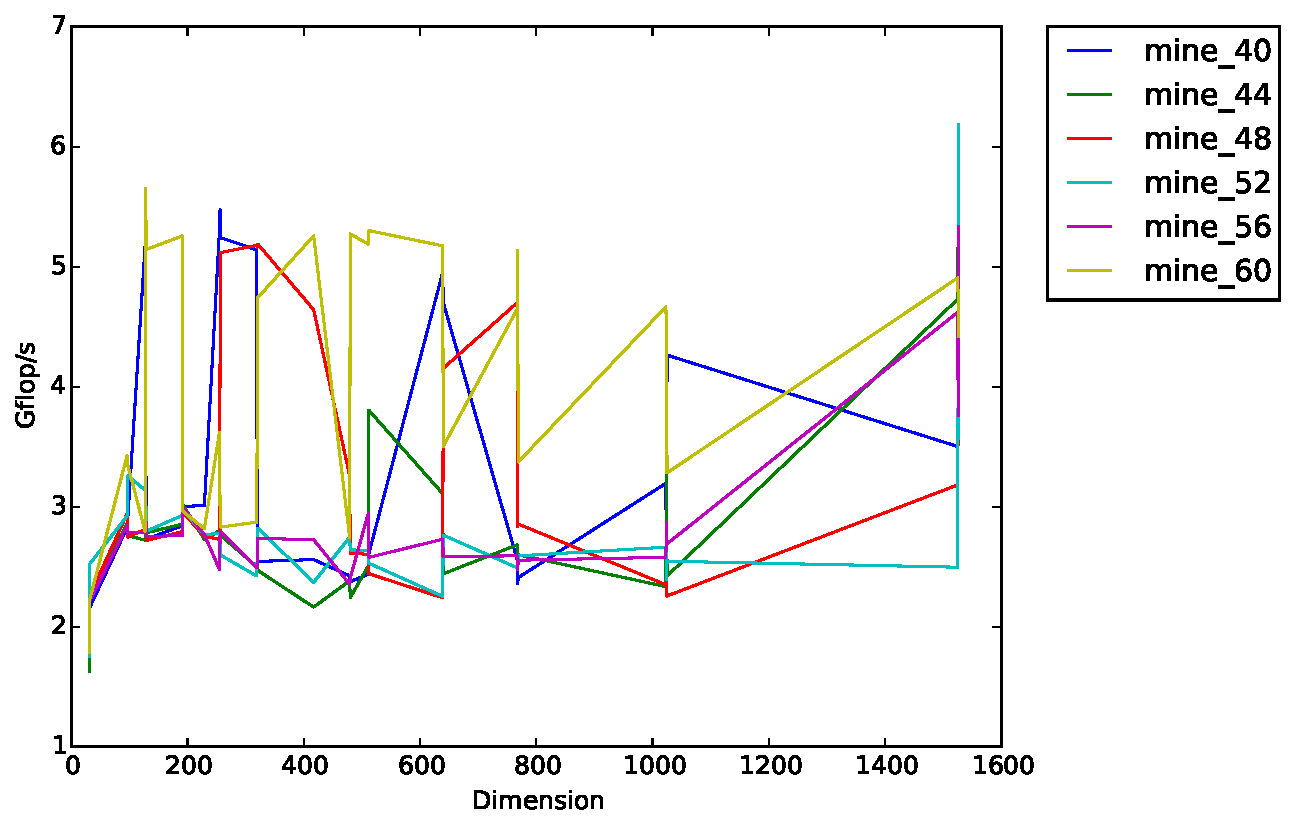
\includegraphics[width=0.85\textwidth] {timing_ijk_jik_4}
        \end{center}
      \label{aload1}
      \caption{blocking with loop order $(i, j, k)\times(j, i, k)$ and copy optimization}
  \end{subfigure}

\end{figure}

\begin{figure}[!ht]
   \begin{subfigure}
      \centering
        \begin{center}
      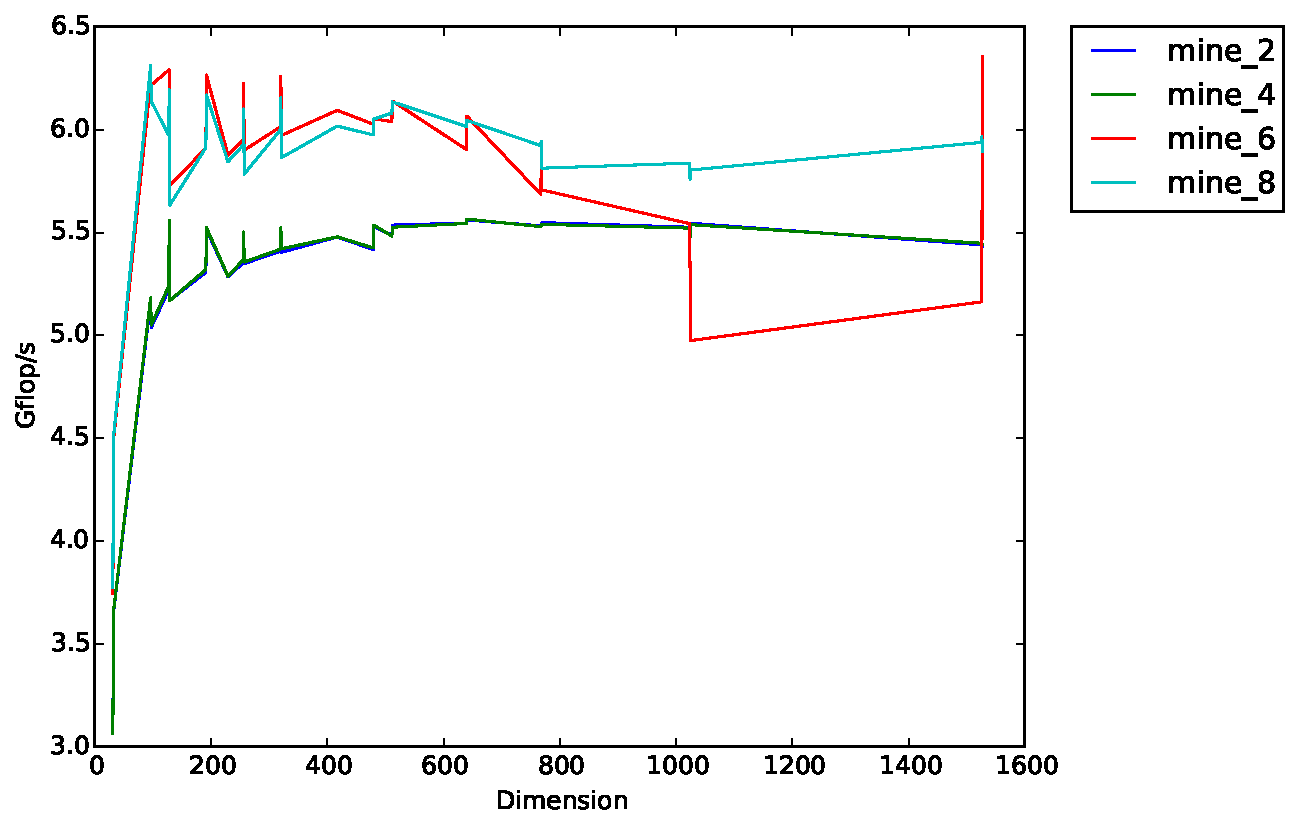
\includegraphics[width=0.85\textwidth] {timing_ijk_jik_5}
        \end{center}
      \label{aload0}
      \caption{blocking with loop order $(i, j, k)\times(j, i, k)$ and copy optimization}
  \end{subfigure}
  \begin{subfigure}
      \centering
        \begin{center}
      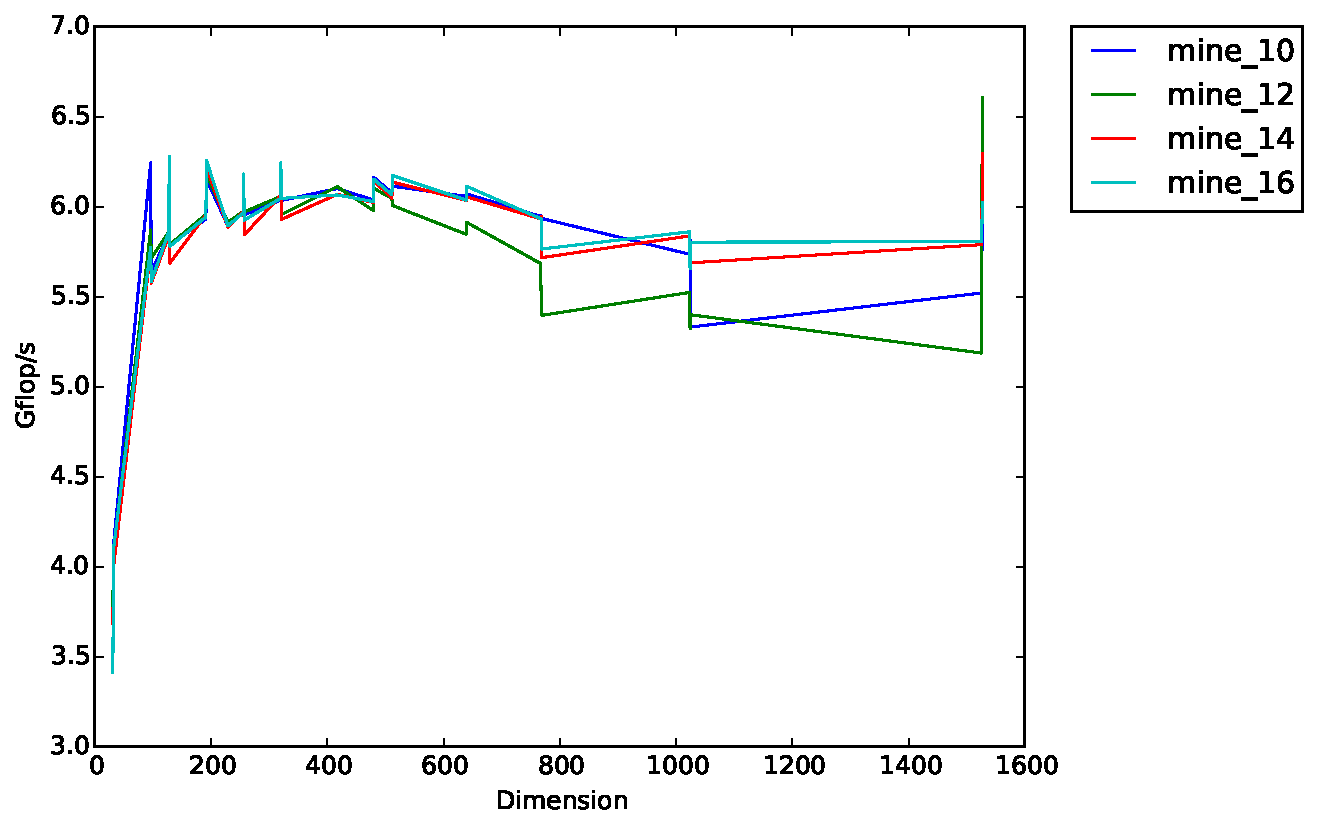
\includegraphics[width=0.85\textwidth] {timing_ijk_jik_6}
        \end{center}
      \label{aload1}
      \caption{blocking with loop order $(i, j, k)\times(j, i, k)$ and copy optimization}
  \end{subfigure}

\end{figure}

\subsection{Future Work}

If we have more time, we would like to try more compiler flags and vector instructions.
\\
We think vector instructions could improve the performance of blocking with looping order $(i, j, k)\times(j, k, i)$ by vectorizing the inner loop of $i$.


\section*{Reference}

(1) David Bindel, Tuning on a single core, Applications of Parallel Computers (CS 5220), Fall 2011.



\end{document}





